\chapter{Filesystem Case Studies}

Chapter xx provided information about features of the main Linux filesystems. This chapter goes a level deeper by describing the internal operation of some of the more important features of each of the most widely used filesystems in the kernel today.

It's not possible to cover everything and some features make good blog posts but topics like ext4 journaling and XXX are popular features and will described in more detail. I have endeavored to choose interesting topics that I think people would find interesting but have not already been covered. For the latter case, I'll provide references. But for popular and well-documented topics such as ext4 journaling, I will provide a different view and, as always, a way to get as hands-on as possible and see for yourself how it works.

For each filesystem, if the contents of on-disk structures for super-blocks, inodes, journals and so on were listed in the book, that would add another hundred pages or more and not be particularly useful. But it's also hard to understand each filesystem without having the information at hand. \textbf{xxx --- need to put it on my website somewhere or reference it if there is good info out there}

\textbf{A forensics tool would be nice to display a bunch of stuff. If it could do multiple filesystems, that would be great}

%%%%%%%%%%%%%%%%%%%%%%%%%%%%%%%%%%%%%%%%%%%%%%%%%%%%%%%%%%%%%%%

\section{The Extended Filesystems}

It's hard to ignore the \textit{Extended Filesystem} which has had a rich and varied history in Linux from the introduction of ext2 in 1993 through to today's journaling ext4.

% https://www.kernel.org/doc/Documentation/filesystems/ext4.txt - official doc
% https://metebalci.com/blog/a-minimum-complete-tutorial-of-linux-ext4-file-system/ - good tutorial
% https://web.mit.edu/tytso/www/linux/ext2intro.html - history up to ext2 - remy card paper
% https://www.sciencedirect.com/science/article/pii/S1742287612000357 - An analysis of Ext4 for digital forensics

%---------------------------------------------------------------------------------------------------------------------------------------------------------------------

\subsection{The ext4 Disk Layout}

XXX

\subsubsection{Extents}

\textbf{xxx --- Another major feature in Ext4 is the use of extents rather than the previously described block mapping method shown in Fig. 2. Extents are more efficient at mapping data blocks of large contiguous files as their structure generally consists of the address of the first physical data block followed by a length.}

xxx

%---------------------------------------------------------------------------------------------------------------------------------------------------------------------

\subsection{ext4 Superblock}

The ext4 superblock is just under 1024 bytes and contains a lot of fields. 

There are several tools to help with analyzing ext4 filesystems:

\begin{itemize}
	\item \cf{dumpe2fs} -- 
	\item \cf{e2fsck} -- 
	\item \cf{tune2fs} -- 
	\item \cf{debugfs} -- 
	\item mactime -- take a look???
\end{itemize}

\noindent
xxx

The The Sleuth Kit (TSK) is a set of useful tools that is used to facilitate the forensic analysis of computer systems. It supports ext2, ext3 and ext4.

%---------------------------------------------------------------------------------------------------------------------------------------------------------------------

\subsection{ext4 Reserved Inodes}

The following inodes are reserved by ext4:

\begin{itemize}
	\setcounter{enumi}{-1}
	\item 0 -- not used.
	\item 1 -- list of defective blocks.
	\item 2 -- root directory.
	\item 3 -- user quota.
	\item 4 -- group quota.
	\item 5 -- boot loader.
	\item 6 -- undelete directory.
	\item 7 -- reserved group descriptors inode. ("resize inode")
	\item 8 -- journal inode.
	\item 9 -- "exclude" inode, for snapshots(?)
	\item 10 -- replica inode, used for some non-upstream feature?
	\item 11 -- traditional first non-reserved inode. Usually this is the \cf{lost+found} directory. See\cf{ s\_first\_ino} in the superblock
\end{itemize}

\noindent
xxx

%---------------------------------------------------------------------------------------------------------------------------------------------------------------------

\subsection{Exploring on-disk ext4 Data Structures}

hard to do all but show how fsdb works so people can look with confidence.

%---------------------------------------------------------------------------------------------------------------------------------------------------------------------

\subsection{ext4 Journaling (jbd2)}

% https://dfrws.org/sites/default/files/session-files/2005_USA_pres-data_hiding_in_journaling_file_systems.pdf 
% See File_System_Journal_Forensics.pdf in Files/Documents/Linux

The ext4 filesystem filesystem implements a \textit{journal} to protect the filesystem against corruption in the case of a system crash. The journal is small and continuous region of disk \textit{reserved inside the filesystem as a place to land "important" data writes on-disk as quickly as possible <- copied}. The default size of the journal is 128 MB.

The following is interesting but copied from the web.

\begin{lstlisting}
# [*\bfseries dumpe2fs /dev/sda2 | grep -i journal*]
Journal inode:            8
Journal backup:           inode blocks
Journal features:         journal_incompat_revoke
Journal size:             32M
Journal length:           8192
Journal sequence:         0x00000662
Journal start:            1
\end{lstlisting}


According to the official documentation:

There are 3 different data modes:

\begin{itemize} 
	\item \cf{writeback mode} --  In \cf{data=writeback} mode, ext4 does not journal data at all. This mode provides a 
		similar level of journaling as that of XFS, JFS, and ReiserFS in its default mode - metadata journaling. 
		A crash+recovery can cause incorrect data to appear in files which were written shortly before the crash. 
		This mode will typically provide the best ext4 performance.
	\item \textbf{ordered mode} --  In \cf{data=ordered} mode, ext4 only officially journals metadata, but it logically 
	groups metadata information related to data changes with the data blocks into a single unit called a transaction. 
	When it's time to write the new metadata out to disk, the associated data blocks are written first. In general, this 
	mode performs slightly slower than writeback but significantly faster than journal mode.
	\item \cf{journal mode} --  \cf{data=journal} mode provides full data and metadata journaling. All new data is written to 
	the journal first, and then to its final location. In the event of a crash, the journal can be replayed, bringing both data 
	and metadata into a consistent state. This mode is the slowest except when data needs to be read from and written 
	to disk at the same time where it outperforms all others modes. Enabling this mode will disable delayed allocation 
	and \cf{O\_DIRECT} support.
\end{itemize} 

\noindent
xxx

\begin{table}[h]
\begin{tabular}{ll}
\parbox[l]{0.6in}{
\includegraphics[scale=0.8]{figures/src-xref.pdf}} & \parbox[l]{4in}{\small{The XXX header file can be found at \cf{fs/ext4/ext4\_jbd2.h} and also at \cf{include/linux/jbd2.h} --- XXX they are different!!!}}
\end{tabular}
\end{table}

\noindent
xxx

%---------------------------------------------------------------------------------------------------------------------------------------------------------------------

\subsection{Analyzing the ext4 Journal}

\begin{lstlisting}
There's a packet in debian called sleuthkit, in which you have 
some  tools like jls or jcat. The jls tool can list all journal 
entries of an ext4  file system, for example:

# jls grafi.img

JBlk    Description
0:      Superblock (seq: 0)
sb version: 4
sb version: 4
sb feature_compat flags 0x00000000
sb feature_incompat flags 0x00000000
sb feature_ro_incompat flags 0x00000000
1:      Allocated Descriptor Block (seq: 2)
2:      Allocated FS Block 161
3:      Allocated Commit Block (seq: 2, sec: 1448889478.49360128)
...
\end{lstlisting}

Need to figure out what we can show

% https://www.usenix.org/legacy/publications/library/proceedings/usenix05/tech/general/full_papers/prabhakaran/prabhakaran_html/main.html

%%%%%%%%%%%%%%%%%%%%%%%%%%%%%%%%%%%%%%%%%%%%%%%%%%%%%%%%%%%%%%%

\section{XFS}

There are approximately 77,000 LOC in \cf{fs/xfs} with the remainder of the tools on 

\subsection{The XFS Disk Layout}

XXX

\begin{figure}[h]
	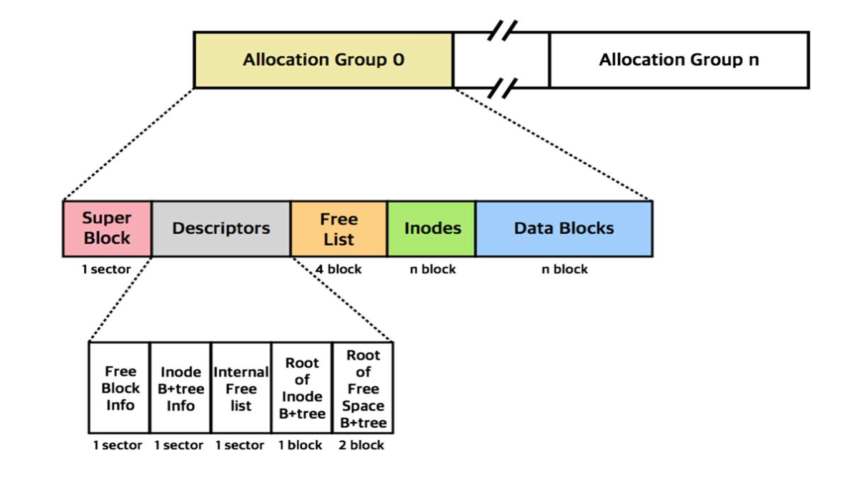
\includegraphics[scale=0.6]{figures/xfs-allocation-group.pdf}
	\centering
	\caption{XFS Allocation Groups}
	\label{fig:xfs-allocation-group}
\end{figure}

Each Allocation Group is divided into four different structures:

\begin{itemize}
	\item Superblock
	\item List of free blocks
	\item Information on allocated and free inodes
	\item Blocks allocated for extension of B-trees
\end{itemize}

\noindent
xxx

The XFS superblock can be seen by ... figure \ref{fig:xfs-superblock} - i like this. find a way to incorprorate some of this with tools for getting to all the main components.

\begin{figure}[h]
	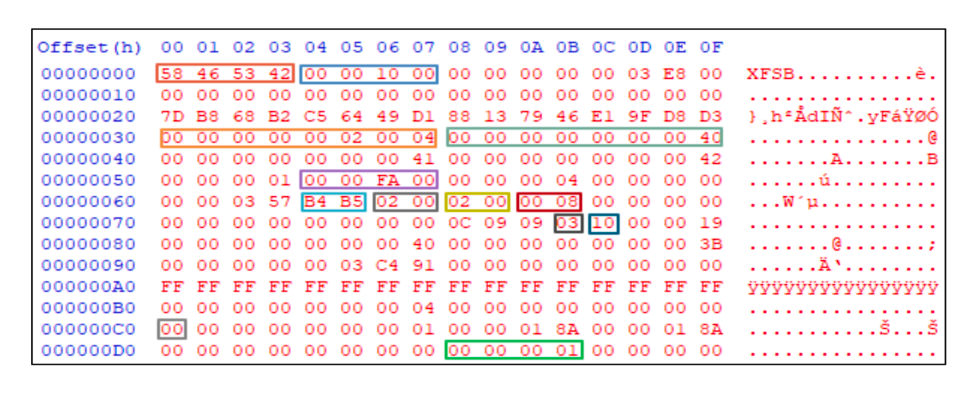
\includegraphics[scale=0.6]{figures/xfs-superblock.pdf}
	\centering
	\caption{XFS Superblock}
	\label{fig:xfs-superblock}
\end{figure}

\subsection{XFS Journaling}

% see Files/Documents/XFS journal analysis.pdf

XXX

\begin{quote}
COPIED --- From the information recorded in superblock, the first block of journal can be reached. Log record begins with a 512 bytes header to document general information of this log record, and it starts with a magic number “0xfeedbabe” to help make sure at the start location of this log record.
\end{quote}

\noindent
xxx

\subsection{Analyzing the XFS Journal}

Need to figure out what we can show

%%%%%%%%%%%%%%%%%%%%%%%%%%%%%%%%%%%%%%%%%%%%%%%%%%%%%%%%%%%%%%%

\section{The btrfs Filesystems}

TBD

\subsection{The btrfs Disk Layout}

XXX

\subsection{btrfs COW vs Journaling}

XXX

%%%%%%%%%%%%%%%%%%%%%%%%%%%%%%%%%%%%%%%%%%%%%%%%%%%%%%%%%%%%%%%

\section{NFS}\label{nfs-chapter}

NFS has gone through several different versions. Rather than dig deep on older versions, this section will focus on version 4 (v4) and make references to earlier versions as needed.

% https://www.kernel.org/doc/ols/2001/nfsv4_ols.pdf - Linux NFS Version 4: Implementation and Administration
% https://docstore.mik.ua/orelly/networking_2ndEd/nfs/ch07_02.htm - old but take a look
% https://www.usenix.org/legacy/event/lisa04/tech/talks/pawlowski.pdf - good overview
% https://www.kernel.org/doc/html/latest/filesystems/nfs/nfs41-server.html - implementation

There are about 80,000 LOC in \cf{fs/nfs} so more than ext4's 60,000 LOC and about half as much code as btfrs 140,000 LOC.

First of all, need a good architecture diagram - can also refer to one in fs chapter.

%----------------------------------------------------------------------------------------------------------------------------------------------------------------------

\subsection{Standardization and Protocols}

xxx

%----------------------------------------------------------------------------------------------------------------------------------------------------------------------

\subsection{Client-side NFS Handling}

xxx

%----------------------------------------------------------------------------------------------------------------------------------------------------------------------

\subsection{Server-side NFS Handling}

xxx

%----------------------------------------------------------------------------------------------------------------------------------------------------------------------

\subsection{NFS Locking}

xxx

%----------------------------------------------------------------------------------------------------------------------------------------------------------------------

\subsection{NFS File Delegation}

xxx

%----------------------------------------------------------------------------------------------------------------------------------------------------------------------

\subsection{Other NFS Implementations}

xxx

% https://github.com/topics/nfs-server - user space implemenation?


%%%%%%%%%%%%%%%%%%%%%%%%%%%%%%%%%%%%%%%%%%%%%%%%%%%%%%%%%%%%%%%

\section{Conclusion}

This chapter described some of the major filesystems in more detail covering topics such as ext4 journaling, NFS client and server side implementation and newer filesystems such as btrfs. It would be possible to write short books on each filesystem so I've been very selective in choosing what to present with the goals of being able to get hands-on to understand the material or to be able to located where relevant information is on the web.

XXX
